\chapter{Cronograma}
\label{cap:cronograma}

O cronograma previsto para a continuidade da pesquisa estende-se até a defesa da dissertação, prevista para julho de 2027. O planejamento considera que parte das etapas iniciais da pesquisa já foi desenvolvida, incluindo a Revisão Sistemática da Literatura, a submissão de artigo derivado dessa etapa e a condução preliminar da campanha experimental.

As atividades restantes concentram-se no refinamento dos resultados experimentais, no aprofundamento da análise estatística, no cálculo de características informacionais dos dados, na construção do modelo quantitativo de apoio à decisão arquitetural, na validação preliminar da abordagem e na redação final da dissertação.


\begin{figure}[htbp]
\centering
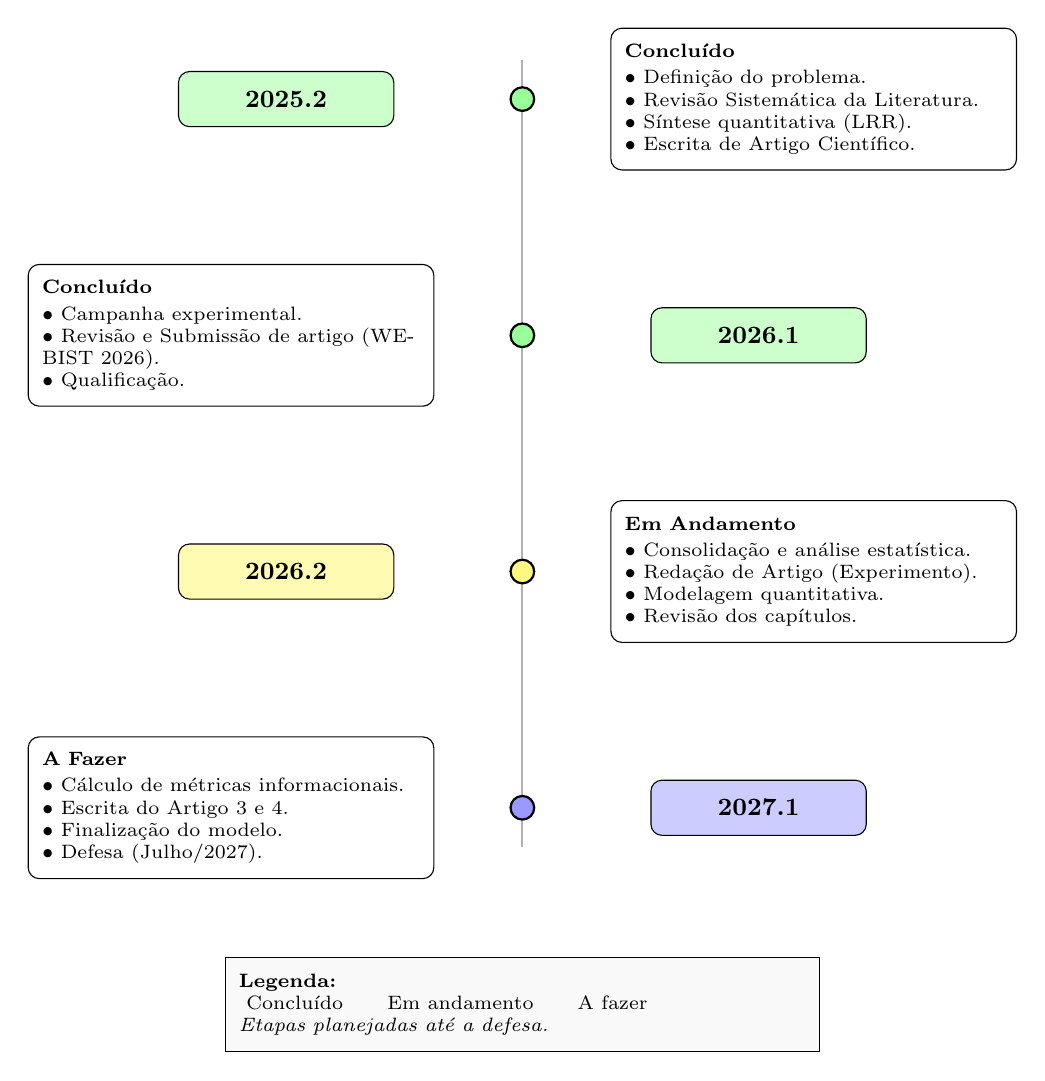
\begin{tikzpicture}[
    periodo/.style={
        rectangle, rounded corners, draw=black, align=center,
        text width=2.5cm, minimum height=0.7cm,
        font=\small\bfseries
    },
    atividade/.style={
        rectangle, rounded corners, draw=black, align=left,
        text width=4.8cm, minimum height=1.8cm,
        font=\scriptsize, fill=white, inner sep=5pt
    },
    legenda/.style={
        rectangle, draw=black, align=left,
        text width=7.2cm, minimum height=1.2cm,
        font=\scriptsize, fill=gray!5, inner sep=5pt
    }
]
% Linha central
\draw[thick, gray!60] (0,0.5) -- (0,-9.5);

% Períodos
\node[periodo, fill=green!20] at (-3,0) {2025.2};
\filldraw[fill=green!40, draw=black, thick] (0,0) circle (0.15);

\node[periodo, fill=green!20] at (3, -3) {2026.1};
\filldraw[fill=green!40, draw=black, thick] (0,-3) circle (0.15);

\node[periodo, fill=yellow!30] at (-3, -6) {2026.2};
\filldraw[fill=yellow!50, draw=black, thick] (0,-6) circle (0.15);

\node[periodo, fill=blue!20] at (3, -9) {2027.1};
\filldraw[fill=blue!40, draw=black, thick] (0,-9) circle (0.15);

% Atividades
\node[atividade] at (3.7,0) {
    \textbf{Concluído}\\[0.5ex]
    $\bullet$ Definição do problema.\\
    $\bullet$ Revisão Sistemática da Literatura.\\
    $\bullet$ Síntese quantitativa (LRR).\\
    $\bullet$ Escrita de Artigo Científico.
};

\node[atividade] at (-3.7, -3) {
    \textbf{Concluído}\\[0.5ex]
    $\bullet$ Campanha experimental.\\
    $\bullet$ Revisão e Submissão de artigo (WEBIST 2026).\\
    $\bullet$ Qualificação.
};

\node[atividade] at (3.7, -6) {
    \textbf{Em Andamento}\\[0.5ex]
    $\bullet$ Consolidação e análise estatística.\\
    $\bullet$ Redação de Artigo (Experimento).\\
    $\bullet$ Modelagem quantitativa.\\
    $\bullet$ Revisão dos capítulos.
};

\node[atividade] at (-3.7, -9) {
    \textbf{A Fazer}\\[0.5ex]
    $\bullet$ Cálculo de métricas informacionais.\\
    $\bullet$ Escrita do Artigo 3 e 4.\\
    $\bullet$ Finalização do modelo.\\
    $\bullet$ Defesa (Julho/2027).
};

% Legenda corrigida (Sem \tikz aninhado)
\node[legenda] at (0,-11.5) {
    \textbf{Legenda:}\\
    $\square$ Concluído \hspace{1em} $\square$ Em andamento \hspace{1em} $\square$ A fazer\\
    \textit{Etapas planejadas até a defesa.}
};
\end{tikzpicture}
\caption{Cronograma das atividades de pesquisa.}
\label{fig:cronograma-visual}
\end{figure}
